\chapter{傅里叶对偶性、动量与自由粒子运动}

\section{从基础到实例}

纠缠处于量子力学的核心，但如今基础已经充分展开，我们可以开始运用它们了。本课程迄今依赖的是刻意选取的小系统：一个自旋、一台可旋转的装置、一份有限的结果清单，以及由重复测量推断出的概率。这些实验在逻辑上比量子力学被发现的历史路径更简单，但它们包含了最低限度的操作要素。

\begin{classroomqa}
\audiencequestion{在量子力学中，什么扮演了牛顿那少量经验起点的角色？}
\lecturerresponse{一个最小模型就是可旋转的自旋装置。制备一个自旋，选择一根轴，按下测量控制键，记录\(+1\)或\(-1\)，并重复实验直到结果频率已知。矢量空间、可观测量、振幅和玻恩定则组织起这些统计结果。历史上，该理论源自远为丰富的原子现象，但从逻辑上说，这个双结果实验就足以揭示其结构。}
\end{classroomqa}

\begin{classroomqa}
\audiencequestion{是否必须对每个物理量，例如自旋或动量，都执行同样的统计程序？}
\lecturerresponse{是的。一个可观测量与一类实验安排及可能结果相联系。一旦指定了态和可观测量，形式体系就预言其分布，但可观测量的物理意义由它如何被测量来锚定。}
\end{classroomqa}

在离开纠缠之前，先前讨论中的一个问题值得给出完整回答。考虑两个电子，具有单态和三重态部分，并把辐射场作为另一个量子子系统包括进来。辐射场有一个真空态\(\ket{0_\gamma}\)和一个单光子态\(\ket{1_\gamma}\)。粒子数本身也可以叠加；并没有规则限制叠加只能发生在固定粒子数的不同态之间。

对于课上讨论的理想化跃迁，一个初始未纠缠的电子态可以写成单态和三重态分量的叠加，
\begin{equation}
\ket{\uparrow\downarrow}
=
\frac{1}{\sqrt{2}}
\left(\ket{S}+\ket{T_0}\right).
\end{equation}
初始没有光子存在时，态为
\begin{equation}
\ket{\Psi(0)}
=
\frac{1}{\sqrt{2}}
\left(\ket{S}+\ket{T_0}\right)
\otimes\ket{0_\gamma}.
\label{eq:l9-initial-radiative-state}
\end{equation}
单态分量不发生发射，仍保持为单态，而激发态的三重态分量可以弛豫到单态并发射一个光子：
\begin{align}
\ket{S}\ket{0_\gamma}
&\longrightarrow
\ket{S}\ket{0_\gamma}, \\
\ket{T_0}\ket{0_\gamma}
&\longrightarrow
\ket{S}\ket{1_\gamma}.
\end{align}
线性性于是给出
\begin{equation}
\ket{\Psi_{\mathrm{final}}}
=
\ket{S}\otimes
\frac{\ket{0_\gamma}+\ket{1_\gamma}}{\sqrt{2}}.
\label{eq:l9-final-radiative-state}
\end{equation}

\begin{figure}[htbp]
\centering
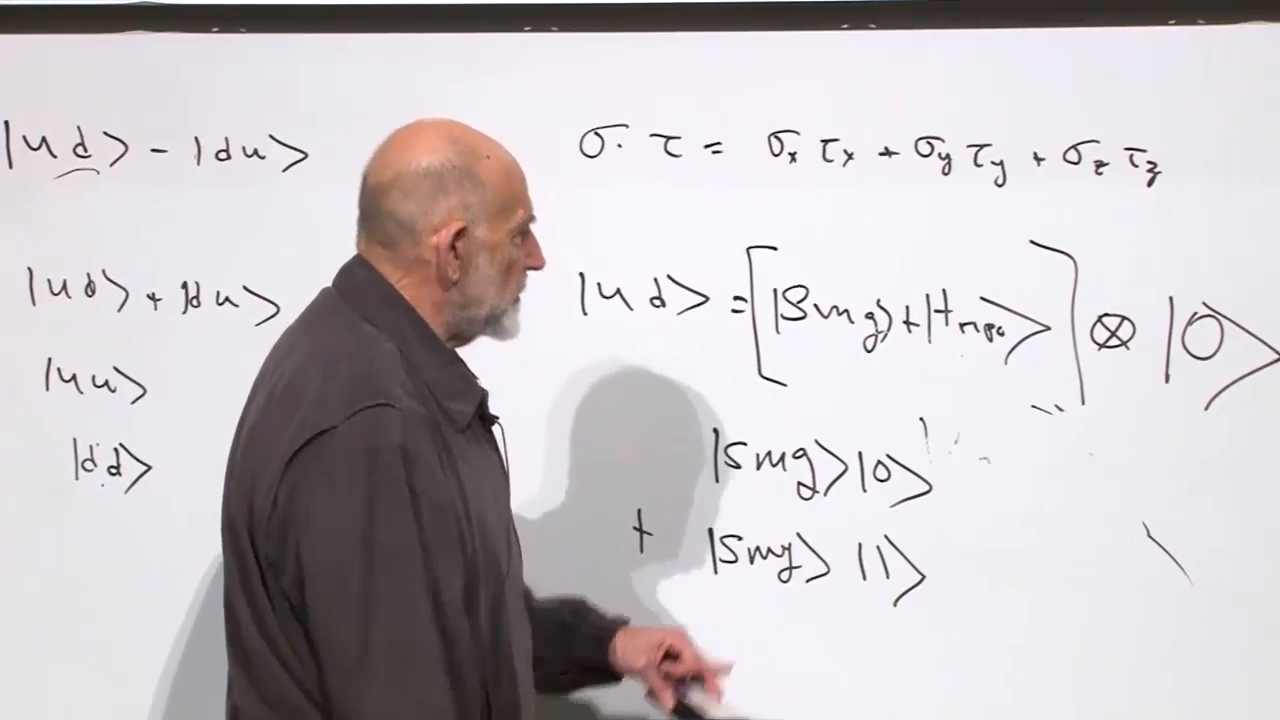
\includegraphics[width=0.88\textwidth]{lecture_09_figure_01.png}
\caption{电子态被分解为单态和三重态分量，并在辐射弛豫之前与光子真空态作张量积。}
\lectureframe{00:05:10}
\end{figure}

最终表达式是电子对与辐射场之间的乘积。两个电子彼此纠缠，因为\(\ket{S}\)是纠缠的，而辐射场则处于零光子和一个光子的叠加态。这个例子之所以微妙，是因为相互作用重新分配了纠缠：初始的电子乘积态演化为纠缠的电子对，然而最终理想化的电子-辐射态却因子化。

\begin{classroomqa}
\audiencequestion{任何入射光子能否逆转该跃迁并使电子退纠缠？}
\lecturerresponse{不能。时间反演过程需要适当的光子态、模式、相位、能量和相互作用历史。把发射出的光子反射回去，只是安排整个封闭系统逆演化的简写，并不是声称任意一个光子都会解除纠缠。}
\end{classroomqa}

\begin{classroomqa}
\audiencequestion{如果没有引入外磁场，是什么导致三重态发射？}
\lecturerresponse{电子彼此相互作用，并与量子化电磁场相互作用。它们依赖于自旋的相互作用使一种自旋构型在能量上更有利，而多余的能量可以作为辐射离开。不需要外部测量装置；这是电子与场组合系统的普通幺正动力学。}
\end{classroomqa}

在解决了这最后一个问题之后，我们现在忘掉自旋，研究最简单的运动问题：一维直线上的一个粒子。

\section{平面波与傅里叶对}

在回到物理学之前，我们需要一段数学插曲。从下式开始
\begin{equation}
e^{ipx}=\cos(px)+i\sin(px).
\end{equation}
在这个阶段，\(p\)只是一个控制振荡速率的实数。该表达式不含时间依赖，因此尚未描述一个运动的波。它被称为平面波，是因为作为\(x\)的函数，它具有熟悉的 sinusoidal 形式。

一大类足够规则的函数都可以分解为这样的模式。我们把注意力限制在行为足够良好、使下面的积分有意义的函数上：它们不允许在空间无穷远处发散，而之后的物理波函数将是平方可积的。采用对称归一化约定时，傅里叶变换对为
\begin{align}
\psi(x)
&=
\int_{-\infty}^{\infty}
\frac{dp}{\sqrt{2\pi}}\,
\widetilde{\psi}(p)e^{ipx},
\label{eq:l9-fourier-forward}\\
\widetilde{\psi}(p)
&=
\int_{-\infty}^{\infty}
\frac{dx}{\sqrt{2\pi}}\,
\psi(x)e^{-ipx}.
\label{eq:l9-fourier-inverse}
\end{align}
系数\(\widetilde{\psi}(p)\)是带有傅里叶标签\(p\)的模式的复振幅。因子\(1/\sqrt{2\pi}\)是约定性的；在每个方向上各放一个，使两个公式看起来互为倒数。指数中的相对负号是本质性的。

\begin{figure}[htbp]
\centering
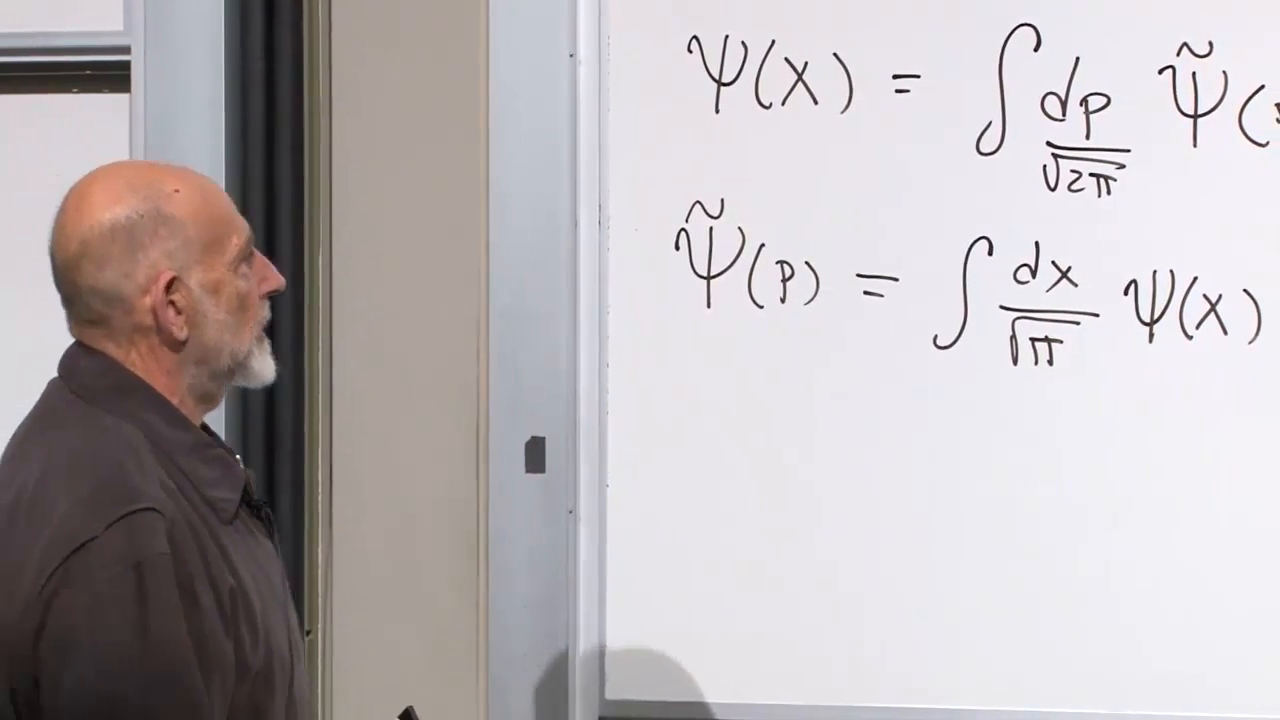
\includegraphics[width=0.88\textwidth]{lecture_09_figure_02.png}
\caption{对称傅里叶变换对：一个函数被分解为平面波，而模式振幅由逆变换恢复。}
\lectureframe{00:14:35}
\end{figure}

\begin{classroomqa}
\audiencequestion{\(\psi(x)\)和\(\widetilde{\psi}(p)\)是否被设定为复数？}
\lecturerresponse{一般来说，是的。一个特殊函数可能恰好是实的，此时它的傅里叶系数满足一个额外的共轭关系，但量子振幅自然是复的，这里不施加任何实性限制。}
\end{classroomqa}

\begin{classroomqa}
\audiencequestion{为什么要使用对称因子\(1/\sqrt{2\pi}\)，而不是把全部\(2\pi\)都放在一个变换中？}
\lecturerresponse{两种约定都是自洽的。对称选择使正变换和逆变换只相差指数中的符号。只要所有相关的归一化都一致地改变，物理预言就不依赖于约定。}
\end{classroomqa}

\(x\)与\(p\)之间的互逆关系已经可见。一个函数通过对另一个变量积分而被分解。目前这还只是傅里叶分析。很快，同一对变量将变成位置和动量。

\section{作为运算的狄拉克{\proseunicodefont δ}}

直观的{\proseunicodefont δ}函数是一个宽度趋于零、高度发散、面积为1的尖峰。这个图像很有用，但运算式定义更可靠。对每一个合适的检验函数\(f\)，
\begin{equation}
\int_{-\infty}^{\infty}
dx\,\delta(x-x')f(x)
=f(x').
\label{eq:l9-delta-sampling}
\end{equation}
三条熟悉的规则表达了同一思想：
\begin{align}
f(x)\delta(x-x')
&=
f(x')\delta(x-x'),
\label{eq:l9-delta-multiplication}\\
\int_{-\infty}^{\infty}dx\,\delta(x-x')
&=1,
\label{eq:l9-delta-area}\\
\int_{-\infty}^{\infty}dx\,\delta(x-x')f(x)
&=f(x').
\end{align}
第一条规则成立，是因为{\proseunicodefont δ}仅在\(x=x'\)处有支集。在第二条规则中，平移尖峰改变了它的位置，但不改变它的面积。把这两条规则结合起来就得到第三条。

\begin{figure}[htbp]
\centering
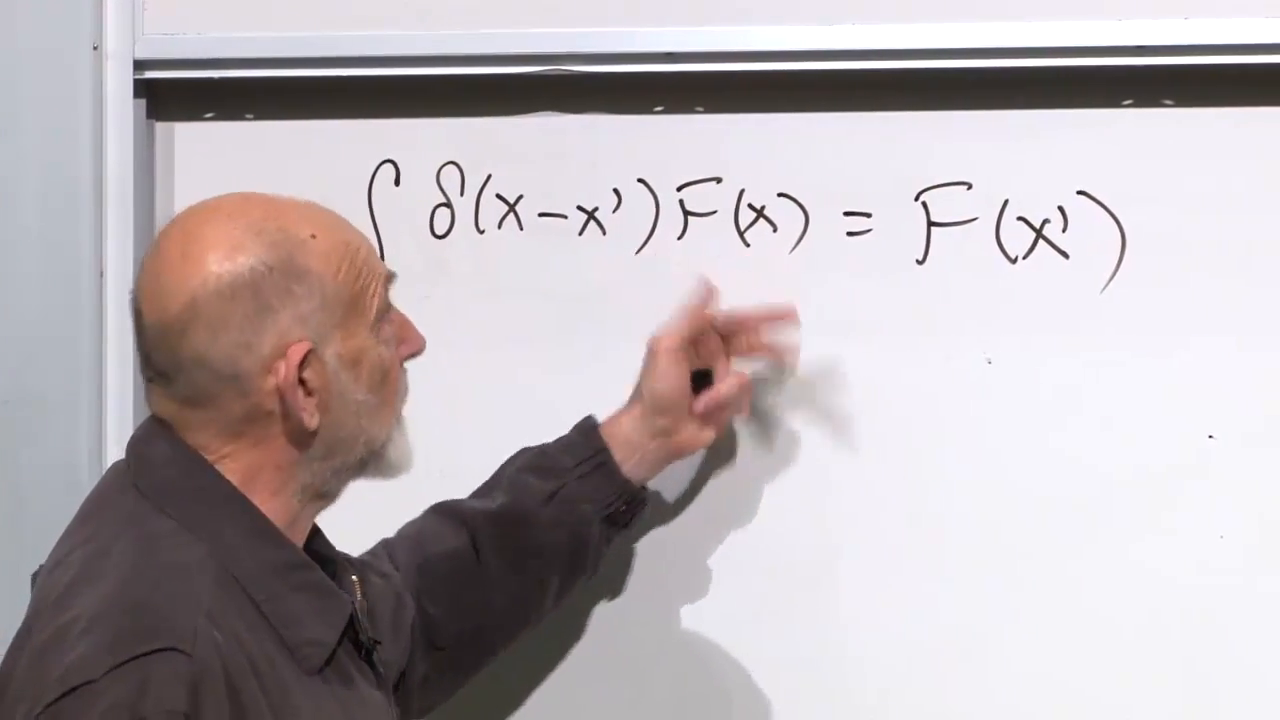
\includegraphics[width=0.88\textwidth]{lecture_09_figure_03.png}
\caption{通过狄拉克{\proseunicodefont δ}对每一个合适函数的作用来刻画它的抽样性质。}
\lectureframe{00:19:45}
\end{figure}

\begin{classroomqa}
\audiencequestion{为什么可以把\(f(x')\)提到\(x\)积分之外？}
\lecturerresponse{积分变量是\(x\)。在该积分过程中，标签\(x'\)是固定的，因此\(f(x')\)相对于\(x\)是常量。剩下的delta积分具有单位面积。}
\end{classroomqa}

{\proseunicodefont δ}不是普通的逐点函数。特别地，试图对它平方会得到一个比原{\proseunicodefont δ}更奇异的对象。它的安全含义是分布式的：方程~\eqref{eq:l9-delta-sampling}规定了它在积分下的作用。

\subsection{{\proseunicodefont δ}的傅里叶表示}

把方程~\eqref{eq:l9-fourier-inverse}代入方程~\eqref{eq:l9-fourier-forward}，并把左边的自变量改名为\(x'\)：
\begin{align}
\psi(x')
&=
\int\frac{dp}{\sqrt{2\pi}}\,
e^{ipx'}
\left[
\int\frac{dx}{\sqrt{2\pi}}\,
\psi(x)e^{-ipx}
\right] \notag\\
&=
\int dx
\left[
\int\frac{dp}{2\pi}
e^{ip(x'-x)}
\right]\psi(x).
\label{eq:l9-fourier-composition}
\end{align}
方括号中的表达式必须对每一个合适的\(\psi\)重现\(\psi(x')\)。与{\proseunicodefont δ}的定义作用相比较，得到
\begin{equation}
\boxed{
\int_{-\infty}^{\infty}
\frac{dp}{2\pi}\,
e^{ip(x'-x)}
=\delta(x'-x)
}.
\label{eq:l9-delta-fourier-x}
\end{equation}

\begin{figure}[htbp]
\centering
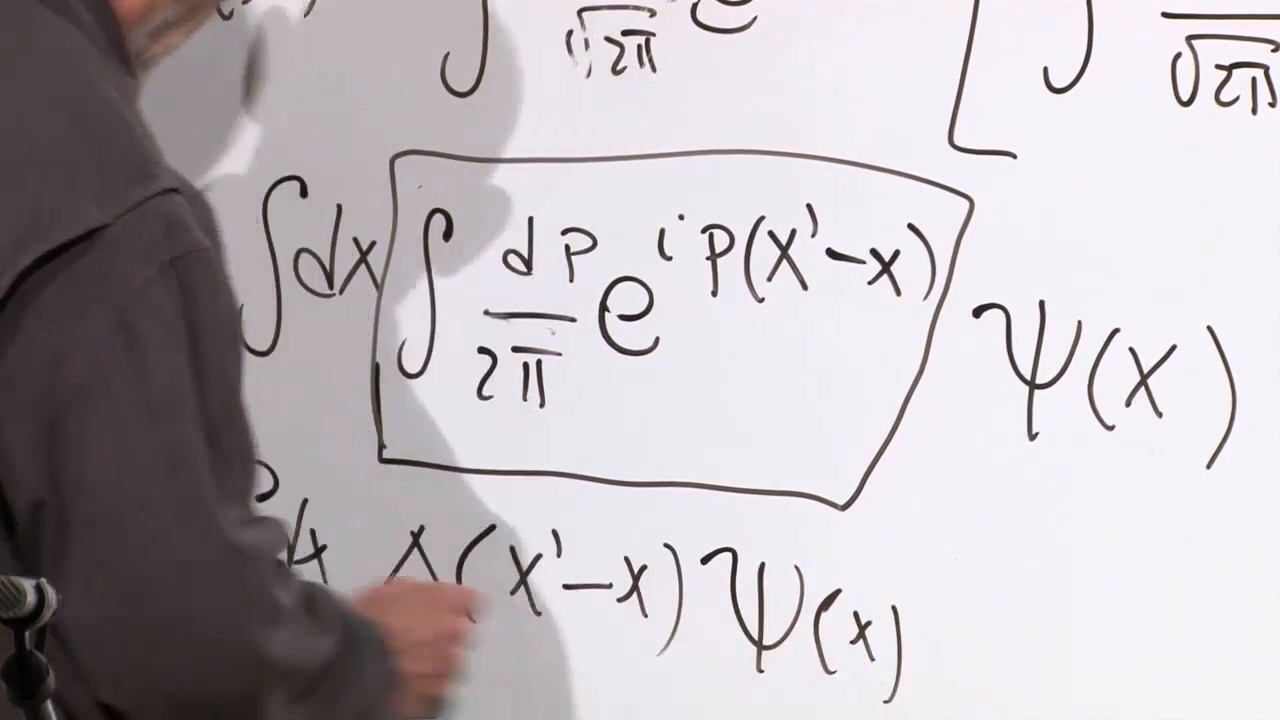
\includegraphics[width=0.88\textwidth]{lecture_09_figure_04.png}
\caption{傅里叶核被隔离在两个变换的复合之中，并通过其抽样作用被识别为狄拉克{\proseunicodefont δ}。}
\lectureframe{00:26:23}
\end{figure}

交换这对互逆变量的名称，得到伴随恒等式
\begin{equation}
\boxed{
\int_{-\infty}^{\infty}
\frac{dx}{2\pi}\,
e^{ix(p-p')}
=\delta(p-p')
}.
\label{eq:l9-delta-fourier-p}
\end{equation}
因此{\proseunicodefont δ}函数是平面波的连续叠加。

\begin{classroomqa}
\audiencequestion{指数在一处写成\(x'-x\)，在另一处写成\(x-x'\)。符号的改变会改变结果吗？}
\lecturerresponse{不会。{\proseunicodefont δ}是偶函数：\(\delta(u)=\delta(-u)\)。因此，反转差值的符号不会改变最终的分布。中间的指数变为其复共轭，但积分后的核仍是同一个{\proseunicodefont δ}。}
\end{classroomqa}

这些操作掩盖了一个收敛性条件。这些振荡积分是分布，而不是绝对收敛的普通积分，交换积分次序需要谨慎。有限的周期区间提供了一个干净的调节器：首先使用离散傅里叶模式和克罗内克正交性，然后让区间无界增大。上面的连续恒等式就是所得的极限。

\section{直线上的粒子}

经典地，相空间中的一个点就确定了状态：
\begin{equation}
(x,p).
\end{equation}
量子力学首先提出的是另一个问题：什么正交归一基定义了状态空间？对每个实位置\(x\)，引入广义本征右矢\(\ket{x}\)。一般态可展开为
\begin{equation}
\ket{\Psi}
=
\int_{-\infty}^{\infty}
dx\,\psi(x)\ket{x},
\qquad
\psi(x)=\braket{x}{\Psi}.
\label{eq:l9-position-expansion}
\end{equation}

\begin{figure}[htbp]
\centering
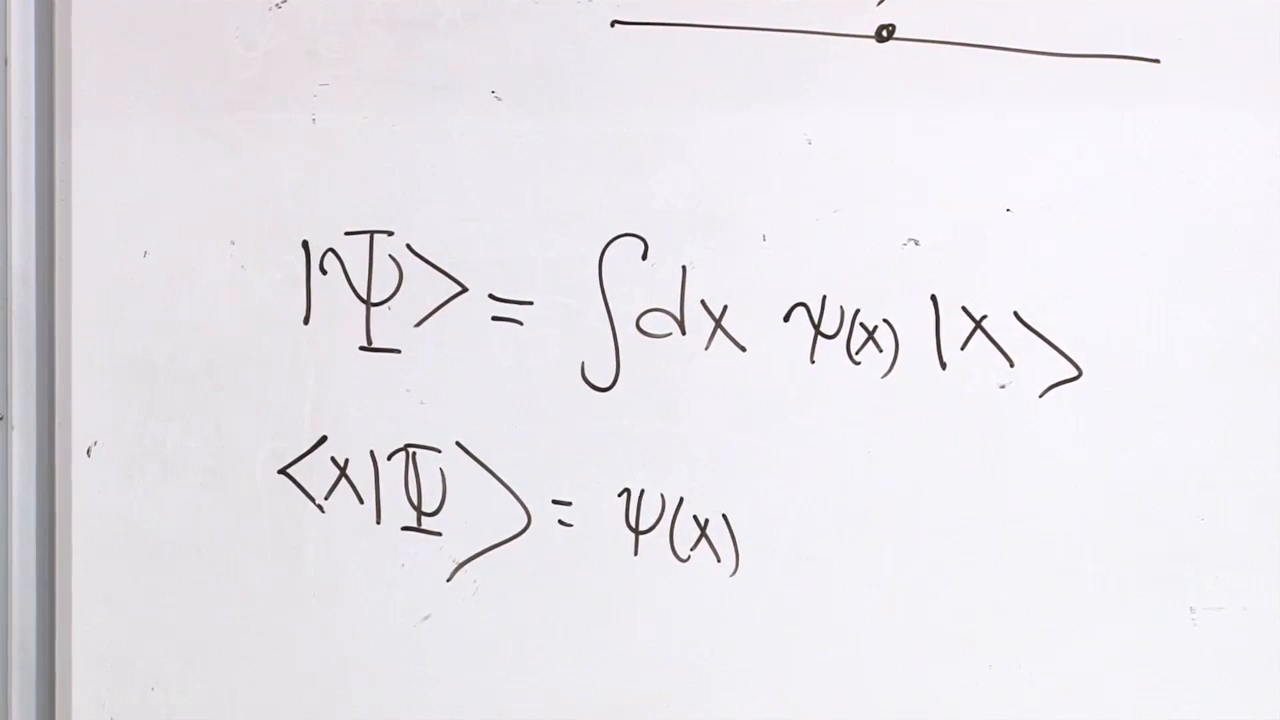
\includegraphics[width=0.88\textwidth]{lecture_09_figure_05.png}
\caption{一般态在连续位置基中的展开，其系数通过向\(\ket{x}\)投影而恢复。}
\lectureframe{00:35:30}
\end{figure}

玻恩规则给出概率密度
\begin{equation}
\rho(x)=|\psi(x)|^2.
\end{equation}
有限区间内的概率为
\begin{equation}
P(a<x<b)=\int_a^b|\psi(x)|^2\,dx,
\end{equation}
而归一化的物理态满足
\begin{equation}
\int_{-\infty}^{\infty}|\psi(x)|^2\,dx=1.
\label{eq:l9-position-normalization}
\end{equation}
连续正交性表示为
\begin{equation}
\braket{x'}{x}=\delta(x-x').
\label{eq:l9-position-delta}
\end{equation}
对两个任意态，内积成为
\begin{equation}
\braket{\Psi}{\Phi}
=
\int_{-\infty}^{\infty}
dx\,\psi^*(x)\phi(x).
\label{eq:l9-position-inner-product}
\end{equation}

\begin{figure}[htbp]
\centering
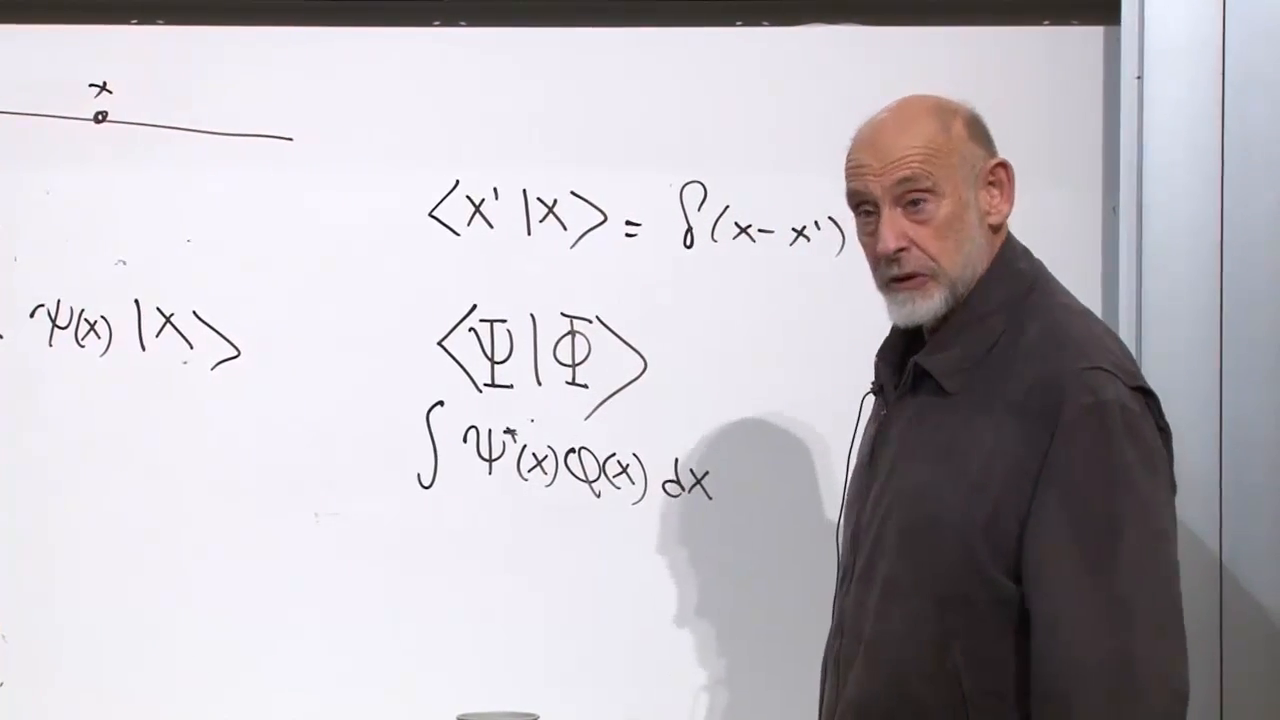
\includegraphics[width=0.88\textwidth]{lecture_09_figure_06.png}
\caption{连续基归一化以及用位置表象写出的波函数内积。}
\lectureframe{00:41:20}
\end{figure}

\begin{classroomqa}
\audiencequestion{为什么仅位置就足够了？加入动量或几乎任何其他变量会是多余的吗？}
\lecturerresponse{对于一维中的一个粒子，完整函数\(\psi(x)\)确定了状态，因此\(p\)的同时确定值将是过多的信息。动量提供另一个完备基，而不是附加到每个\(\ket{x}\)上的额外标签。在更多维中，相容的信息可以混合：例如，\(X\)和\(P_y\)对易，可以标记一个联合基。限制涉及的是不对易对，而不是符号的数目本身。}
\end{classroomqa}

\begin{classroomqa}
\audiencequestion{动量也能提供一个完备基并通过位置展开吗？}
\lecturerresponse{能。动量基是完备的，其系数通过傅里叶变换与位置系数相联系。这一关系是本讲的核心构造。}
\end{classroomqa}

\section{位置表象中的位置}

抽象算符作用于态矢量。一旦选定基，同一作用就成为对波函数的具体操作。在位置表象中，位置算符\(X\)通过乘法作用：
\begin{equation}
(X\psi)(x)=x\psi(x).
\label{eq:l9-position-operator}
\end{equation}

定域于\(x_0\)的态由广义波函数\(\delta(x-x_0)\)表示。施加\(X\)给出
\begin{align}
X\delta(x-x_0)
&=
x\delta(x-x_0) \notag\\
&=
x_0\delta(x-x_0),
\label{eq:l9-position-eigenfunction}
\end{align}
其中使用了方程~\eqref{eq:l9-delta-multiplication}。因此\(\delta(x-x_0)\)是\(X\)的本征函数，本征值为\(x_0\)。

\begin{figure}[htbp]
\centering
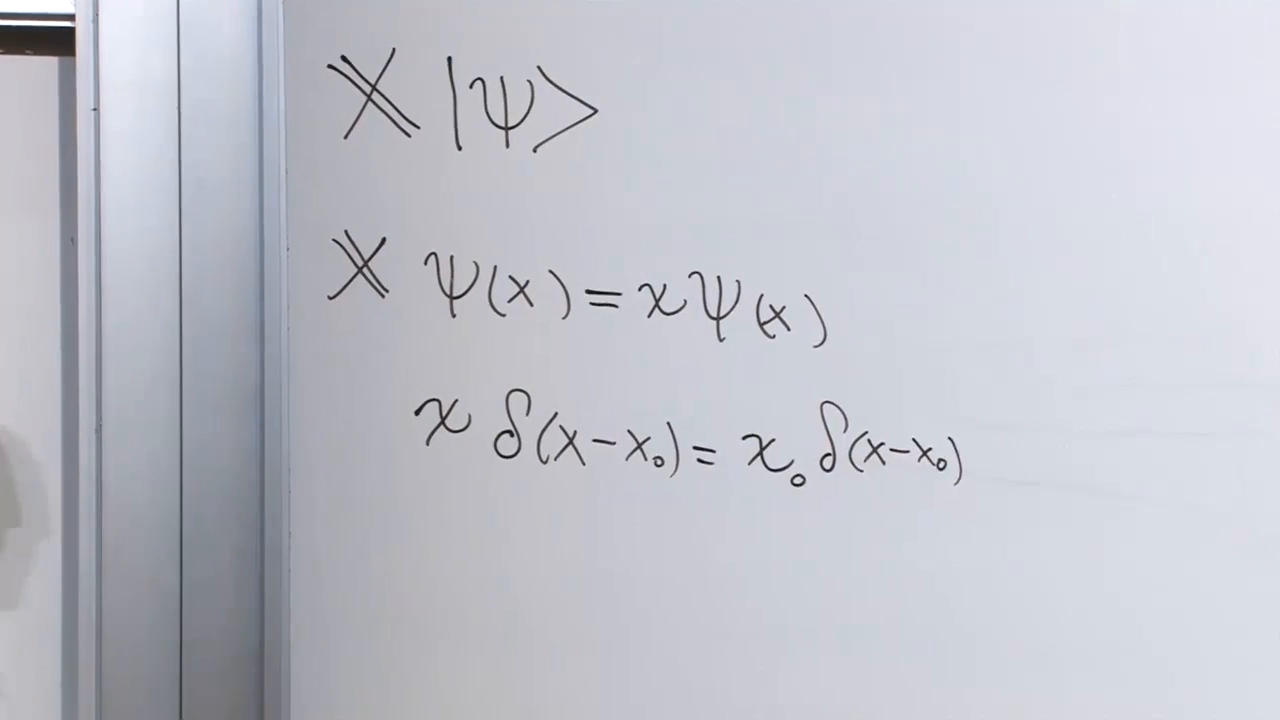
\includegraphics[width=0.88\textwidth]{lecture_09_figure_07.png}
\caption{乘以\(x\)将{\proseunicodefont δ}定域态变为\(x_0\)乘以自身，证明它是位置本征函数。}
\lectureframe{00:45:50}
\end{figure}

\(\ket{x_0}\)及其{\proseunicodefont δ}函数代表都不是在通常平方可积意义下归一化为1的。它是{\proseunicodefont δ}归一化的。物理的定域态是有限波包，而精确本征态则充当广义基矢量。

\section{动量本征函数}

上一讲发现微分是反厄米的，而乘以\(-i\)使其成为厄米的。恢复单位，定义
\begin{equation}
P=-i\hbar\frac{d}{dx},
\qquad
(P\psi)(x)
=
-i\hbar\frac{d\psi}{dx}.
\label{eq:l9-momentum-operator}
\end{equation}
这是适当定义域上的一个合法可观测量。它与物理动量的等同将通过其谱、波长以及在动力学中的作用来检验。

对动量本征值\(p\)，求解
\begin{equation}
P\psi_p=p\psi_p,
\end{equation}
或
\begin{equation}
-i\hbar\frac{d\psi_p}{dx}=p\psi_p.
\end{equation}
解为
\begin{equation}
\psi_p(x)=A e^{ipx/\hbar}.
\label{eq:l9-momentum-eigenfunction}
\end{equation}

\begin{figure}[htbp]
\centering
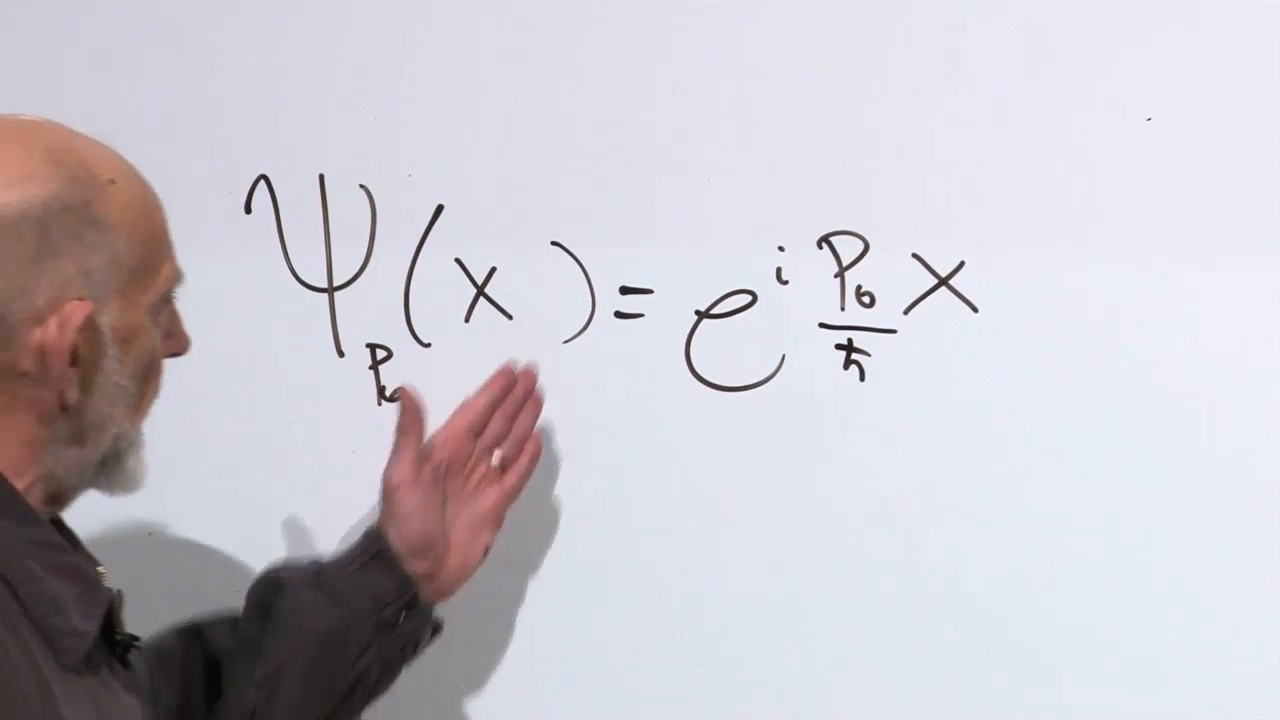
\includegraphics[width=0.88\textwidth]{lecture_09_figure_08.png}
\caption{确定动量态的位置空间代表是平面波\(e^{ipx/\hbar}\)。}
\lectureframe{00:51:45}
\end{figure}

波长\(\lambda\)是使相位推进\(2\pi\)的位移：
\begin{equation}
\frac{p\lambda}{\hbar}=2\pi,
\qquad
\lambda=\frac{2\pi\hbar}{p}.
\label{eq:l9-de-broglie}
\end{equation}
因此较大的动量对应较短的波长。

{\proseunicodefont δ}归一化确定常数：
\begin{equation}
\psi_p(x)
=
\frac{1}{\sqrt{2\pi\hbar}}e^{ipx/\hbar}.
\label{eq:l9-normalized-momentum-eigenfunction}
\end{equation}
确实，
\begin{align}
\braket{p'}{p}
&=
\int_{-\infty}^{\infty}
dx\,
\psi_{p'}^*(x)\psi_p(x) \notag\\
&=
\int_{-\infty}^{\infty}
\frac{dx}{2\pi\hbar}
e^{i(p-p')x/\hbar} \notag\\
&=
\delta(p-p').
\label{eq:l9-momentum-normalization}
\end{align}
在选取\(\hbar=1\)的单位后，这些公式变为
\begin{equation}
\psi_p(x)=\frac{1}{\sqrt{2\pi}}e^{ipx},
\qquad
\int\frac{dx}{2\pi}e^{i(p-p')x}
=\delta(p-p').
\end{equation}

\begin{classroomqa}
\audiencequestion{当振荡积分在通常意义下不收敛时，怎么能对\(p\neq p'\)宣布它为零？}
\lecturerresponse{本讲采取一种受控的捷径。将系统置于有限周期区间上。允许的动量于是形成离散集合，指数函数按通常意义正交，每个归一化都是有限的。只有在此计算之后，才应让区间趋于无穷，将克罗内克{\proseunicodefont δ}变为狄拉克{\proseunicodefont δ}。}
\end{classroomqa}

\begin{classroomqa}
\audiencequestion{同样的收敛问题会影响{\proseunicodefont δ}函数的傅里叶变换推导吗？}
\lecturerresponse{会。出于同样的原因，那里交换积分次序是形式上的。有限盒推导或分布的语言提供了被省略的严格性。这一捷径是可接受的，因为正规化后的计算具有所述连续极限。}
\end{classroomqa}

\section{动量表象}

有两个对象不可混淆。方程~\eqref{eq:l9-normalized-momentum-eigenfunction}中的函数\(\psi_p(x)\)是特定本征态\(\ket{p}\)在位置空间中的代表。相比之下，任意态\(\ket{\Psi}\)的动量空间波函数为
\begin{equation}
\widetilde{\psi}(p)=\braket{p}{\Psi}.
\label{eq:l9-momentum-wavefunction}
\end{equation}
代入\(\bra{p}\)与\(\ket{\Psi}\)的位置空间波函数：
\begin{align}
\widetilde{\psi}(p)
&=
\int_{-\infty}^{\infty}
dx\,
\braket{p}{x}\braket{x}{\Psi} \notag\\
&=
\int_{-\infty}^{\infty}
\frac{dx}{\sqrt{2\pi\hbar}}\,
e^{-ipx/\hbar}\psi(x).
\label{eq:l9-position-to-momentum}
\end{align}
这正是傅里叶变换。反过来，
\begin{equation}
\psi(x)
=
\int_{-\infty}^{\infty}
\frac{dp}{\sqrt{2\pi\hbar}}\,
\widetilde{\psi}(p)e^{ipx/\hbar}.
\label{eq:l9-momentum-to-position}
\end{equation}

\begin{figure}[htbp]
\centering
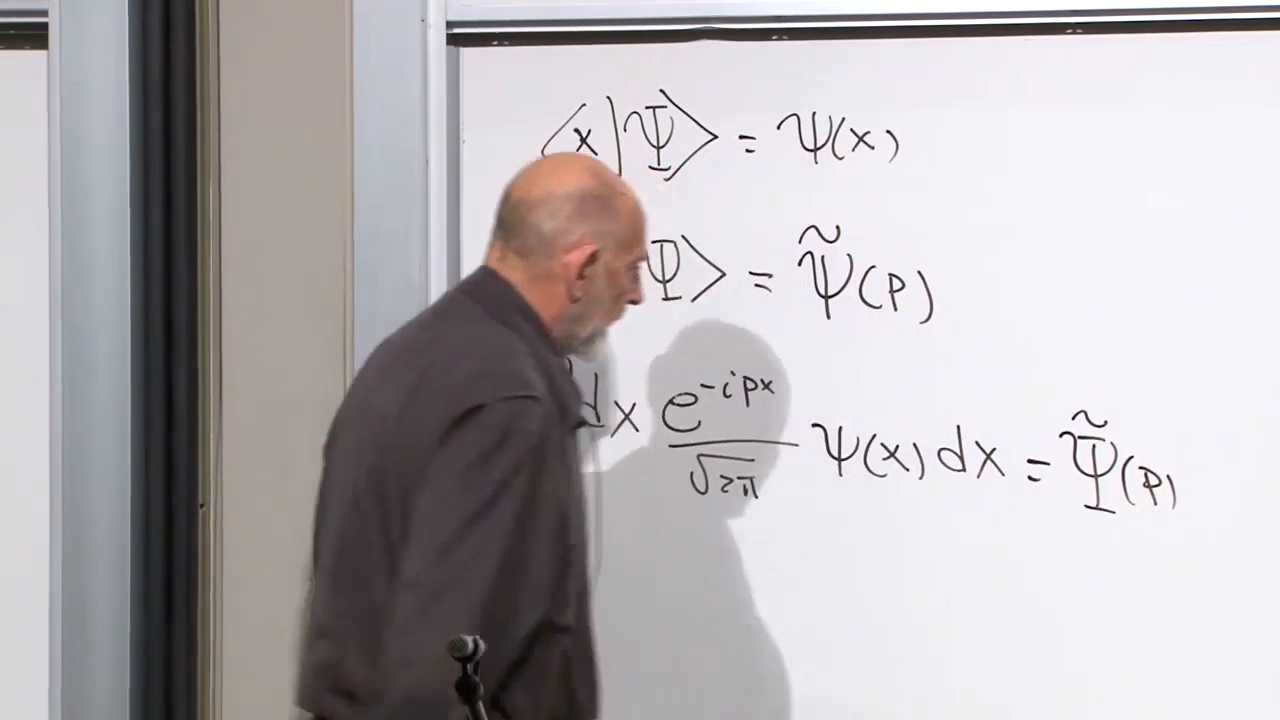
\includegraphics[width=0.88\textwidth]{lecture_09_figure_09.png}
\caption{向\(\ket{p}\)的投影将位置空间波函数变为其傅里叶变换\(\widetilde{\psi}(p)\)。}
\lectureframe{01:05:50}
\end{figure}

测得动量\(p\)的概率密度为
\begin{equation}
\widetilde{\rho}(p)
=
|\widetilde{\psi}(p)|^2,
\qquad
\int_{-\infty}^{\infty}
|\widetilde{\psi}(p)|^2\,dp=1.
\end{equation}
因此，一个位置空间波函数所含的信息足以同时预言位置测量与动量测量的结果。要得到动量概率，只需对\(\psi(x)\)作傅里叶变换，再取结果的模平方。

在动量表象中，两者的角色互换：
\begin{equation}
(P\widetilde{\psi})(p)
=
p\widetilde{\psi}(p),
\qquad
(X\widetilde{\psi})(p)
=
i\hbar\frac{d\widetilde{\psi}}{dp}.
\label{eq:l9-operators-in-p}
\end{equation}
与\(P=-i\hbar\,d/dx\)的符号差异源于傅里叶变换对中相反的符号。

\begin{classroomqa}
\audiencequestion{时间是否像位置与动量共轭那样，是与能量共轭的算符？}
\lecturerresponse{时间通常被视为标记态演化的外部参数，而不是系统希尔伯特空间上一个普遍的自伴算符。物理时钟确实有可观测的读数，提高时钟的时间分辨率也会带来能量上的后果，但时间-能量关系比位置-动量对需要更细致的处理，此处不予展开。}
\end{classroomqa}

\begin{classroomqa}
\audiencequestion{还存在哪些其他共轭对？}
\lecturerresponse{角与相应的角动量提供了一个重要例子，但由于角具有周期性，需要附加整体性的限定条件。在场论中，场与其正则动量共轭。温度与压强是热力学变量，而不是一对正则量子共轭量。一般原理由正则变量及其对易关系给出，而不是由任意一对可测量量给出。}
\end{classroomqa}

\begin{classroomqa}
\audiencequestion{在离散理论中，算符作用于右矢和波函数只不过是在列出系数。在连续理论中这一点改变了吗？}
\lecturerresponse{没有。波函数是抽象右矢在选定基下的坐标列。作用于有限列的矩阵与作用于函数的微分或积分算符，是同一个抽象运算的两种具体表示。连续标号改变的是记号，而不是逻辑。}
\end{classroomqa}

\subsection{作为傅里叶事实的不确定性}

具有确定动量的态完全离域：
\begin{equation}
|\psi_p(x)|^2=\text{constant}.
\end{equation}
其动量是尖锐的，但位置均匀地铺展在整条直线上。更一般地说，傅里叶对不可能同时都很窄。把\(\widetilde{\psi}(p)\)集中到很小的动量范围内，就迫使\(\psi(x)\)延展到很大的区域；而要使\(\psi(x)\)局域化，则需要很宽的动量范围。

本讲尚未推导定量不等式
\begin{equation}
\Delta X\,\Delta P\geq\frac{\hbar}{2}.
\end{equation}
它当前要说明的是结构性的要点：不确定性原理已经编码在傅里叶变换的倒易几何之中。这是在不兼容的自旋基之间变换的连续类比。

\section{哈密顿量生成时间演化}

哈密顿量\(H\)是厄米的，代表能量，并生成幺正时间演化。含时的Schr\"odinger方程为
\begin{equation}
i\hbar\frac{d}{dt}\ket{\Psi(t)}
=
H\ket{\Psi(t)}.
\label{eq:l9-abstract-schrodinger}
\end{equation}
在位置表象中，
\begin{equation}
i\hbar\frac{\partial\psi(x,t)}{\partial t}
=
H\psi(x,t),
\label{eq:l9-position-schrodinger}
\end{equation}
其中右端表示哈密顿量作用于该函数时所选取的位置空间表示。

\subsection{一个刻意选取的简单线性哈密顿量}

取
\begin{equation}
H=cP.
\label{eq:l9-linear-hamiltonian}
\end{equation}
这不是通常的非相对论自由粒子哈密顿量。之所以选取它，是因为每一步都可以直接看出。

\begin{figure}[htbp]
\centering
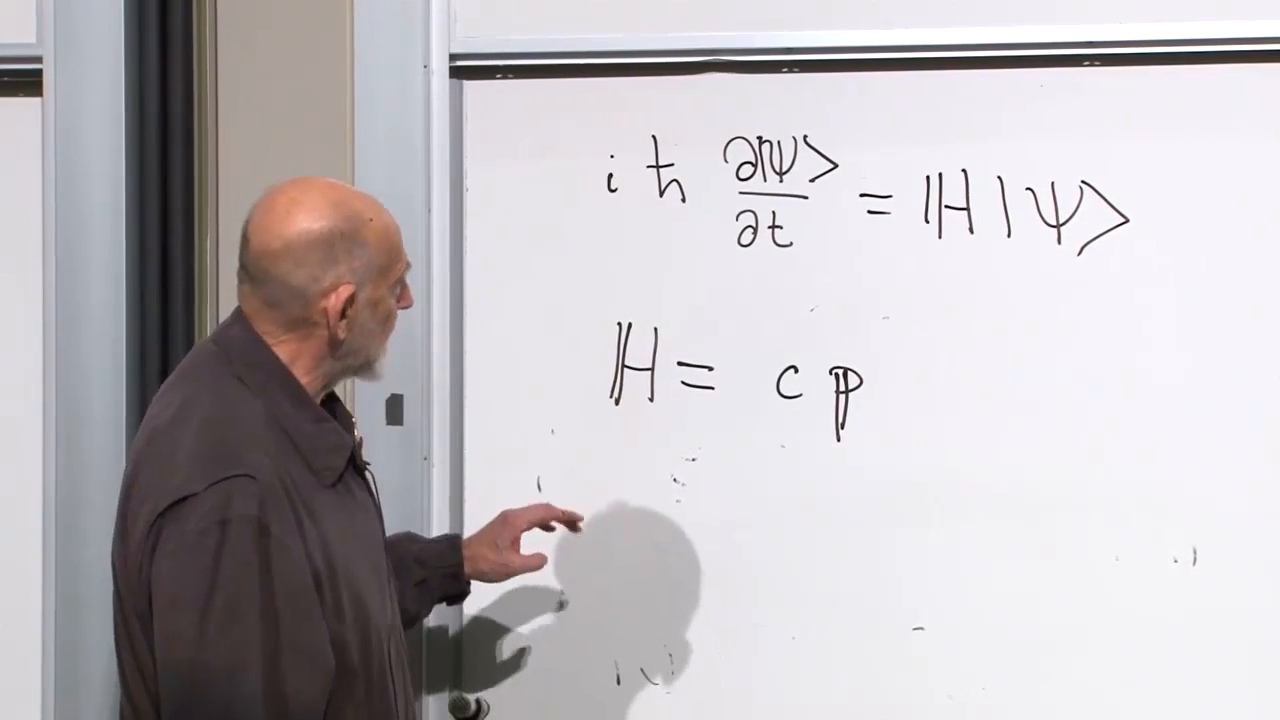
\includegraphics[width=0.88\textwidth]{lecture_09_figure_10.png}
\caption{Schr\"odinger方程与线性哈密顿量\(H=cP\)，后者被选作粒子演化的最简单例子。}
\lectureframe{01:17:45}
\end{figure}

利用\(P=-i\hbar\,\partial_x\)，
\begin{align}
i\hbar\frac{\partial\psi}{\partial t}
&=
c\left(-i\hbar\frac{\partial}{\partial x}\right)\psi, \notag\\
\frac{\partial\psi}{\partial t}
&=
-c\frac{\partial\psi}{\partial x},
\end{align}
或
\begin{equation}
\frac{\partial\psi}{\partial t}
+c\frac{\partial\psi}{\partial x}=0.
\label{eq:l9-transport-equation}
\end{equation}

\begin{figure}[htbp]
\centering
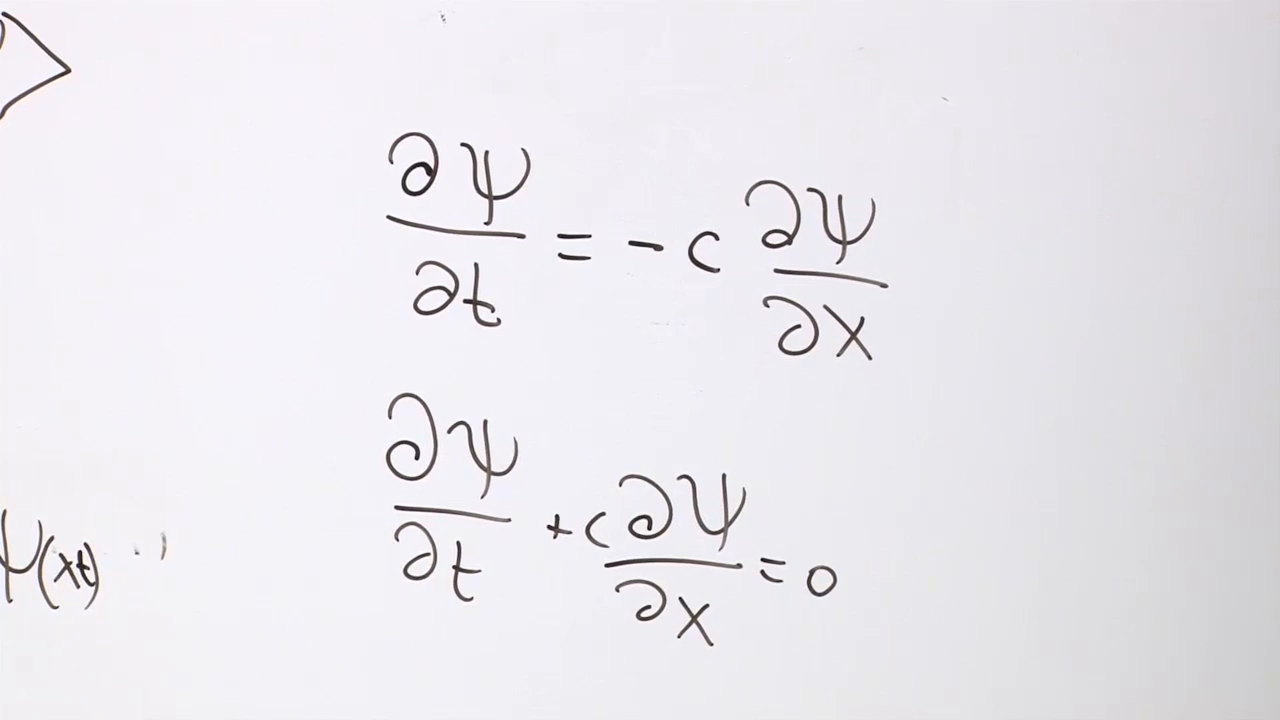
\includegraphics[width=0.88\textwidth]{lecture_09_figure_11.png}
\caption{线性哈密顿量将Schr\"odinger方程化为了一阶输运方程。}
\lectureframe{01:20:05}
\end{figure}

通解为
\begin{equation}
\psi(x,t)=f(x-ct),
\label{eq:l9-rigid-translation}
\end{equation}
其中\(f\)是任意可归一化的初始剖面。在\(t=0\)时，剖面为\(f(x)\)。在更晚的时刻，每一特征都向右平移了\(ct\)。复波函数、它的实部与虚部以及它的概率密度都保持各自的形状：
\begin{equation}
|\psi(x,t)|^2=|f(x-ct)|^2.
\end{equation}
因此，
\begin{equation}
\expect{X}_t=\expect{X}_0+ct.
\end{equation}

选择符号 \(c\) 是为了让人联想到光速。该模型类似于一个一维手性无质量激发：每个允许的分量都以一个速率沿一个方向运动。它并不是一个完整的光子理论。具有固定声速的低能一维声子提供了另一种类比。由于 \(E=cp\)，允许 \(p\) 的两种符号也就允许负能量，这再次表明这是一个刻意受限的教学模型。

\begin{classroomqa}
\audiencequestion{如果把 \(c\) 换成该粒子的速度，\(H=cP\) 还能描述任何自由粒子吗？}
\lecturerresponse{不能。\(H=cP\) 中的固定系数表明每个动量分量都具有相同的速度。对于非相对论粒子，速度为 \(p/m\)，因此它依赖于动量。用 \(v=p/m\) 写出 \(vP\) 后，它不再对 \(P\) 线性；这指向二次型哈密顿量。}
\end{classroomqa}

\begin{classroomqa}
\audiencequestion{普通自由运动电子的波函数难道不应该只是刚性平移吗？}
\lecturerresponse{只有非常特殊的色散关系才会使任意轮廓都发生刚性平移。普通自由电子波包包含许多动量分量，它们的相位以不同速率演化。其中心会移动，但其形状通常会扩散。}
\end{classroomqa}

\subsection{经典对比}

对于经典哈密顿量 \(H=cp\)，哈密顿方程给出
\begin{equation}
\dot{x}=\frac{\partial H}{\partial p}=c,
\qquad
\dot{p}=-\frac{\partial H}{\partial x}=0.
\label{eq:l9-linear-hamilton-equations}
\end{equation}

\begin{figure}[htbp]
\centering
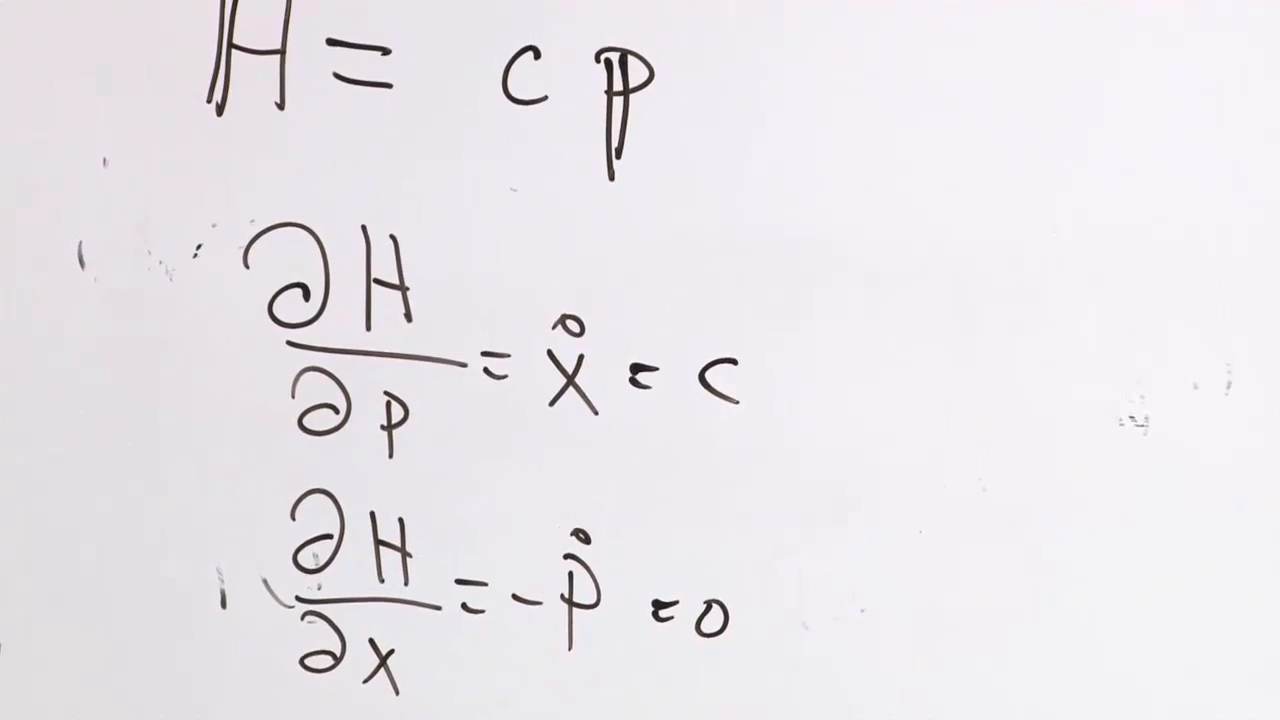
\includegraphics[width=0.88\textwidth]{lecture_09_figure_12.png}
\caption{\(H=cp\) 的哈密顿方程：恒定的向右速度与守恒的动量。}
\lectureframe{01:25:20}
\end{figure}

量子概率分布及其期望值遵循同样的基本运动。这一一致是第一个具体提醒：由经典哈密顿量构建的量子演化应当在适当意义上再现经典方程。

\section{非相对论自由粒子}

对于质量为 \(m\) 且不受力的普通粒子，经典动能为
\begin{equation}
H=\frac{p^2}{2m}.
\end{equation}
该二次型对 \(p\) 和 \(-p\) 的处理是对称的，因此向左运动和向右运动的粒子具有相同的正能量。量子化将 \(p\) 替换为算符 \(P\)：
\begin{equation}
H=\frac{P^2}{2m}.
\label{eq:l9-free-hamiltonian}
\end{equation}
将 \(P=-i\hbar\,\partial_x\) 代入 Schr\"odinger 方程：
\begin{align}
i\hbar\frac{\partial\psi}{\partial t}
&=
\frac{1}{2m}
\left(-i\hbar\frac{\partial}{\partial x}\right)^2
\psi \notag\\
&=
-\frac{\hbar^2}{2m}
\frac{\partial^2\psi}{\partial x^2}.
\label{eq:l9-free-schrodinger}
\end{align}

\begin{figure}[htbp]
\centering
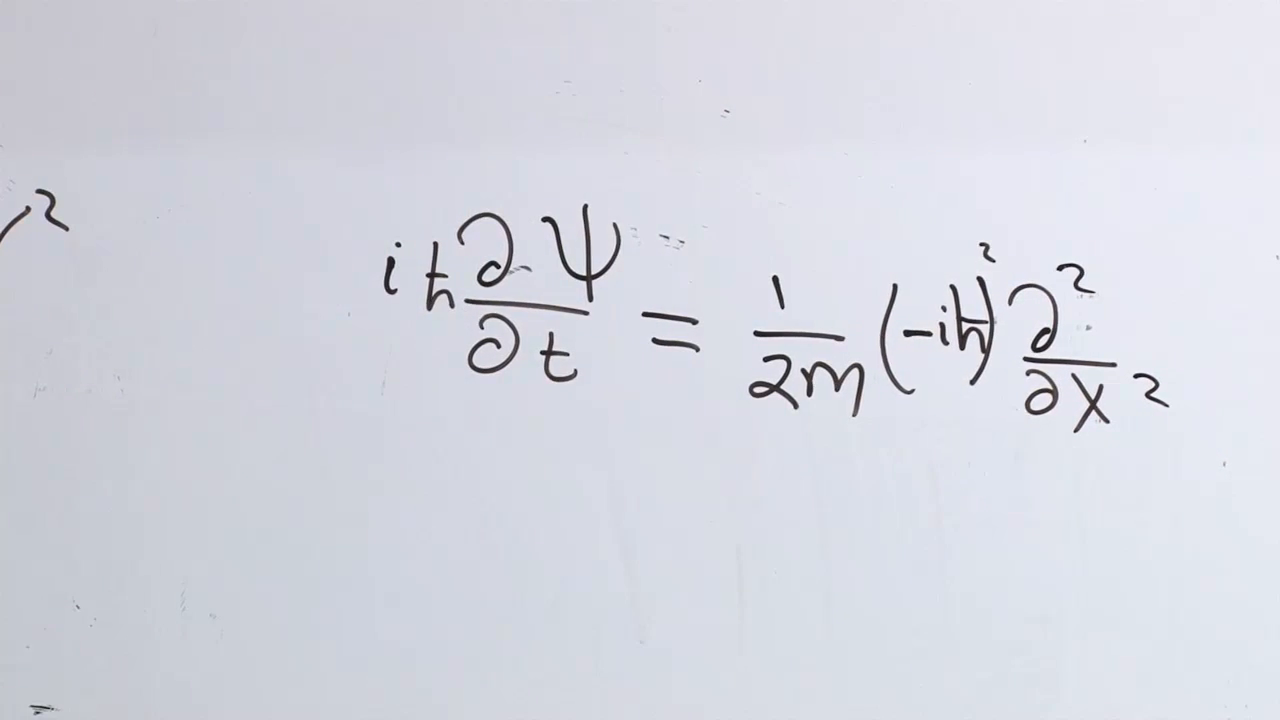
\includegraphics[width=0.88\textwidth]{lecture_09_figure_13.png}
\caption{由 \(H=P^2/(2m)\) 和 \(P=-i\hbar\,\partial_x\) 得到的自由粒子 Schr\"odinger 方程。}
\lectureframe{01:33:50}
\end{figure}

动量为 \(p\) 的平面波分量具有能量
\begin{equation}
E(p)=\frac{p^2}{2m}.
\end{equation}
与线性情形 \(E=cp\) 不同，该色散关系的斜率依赖于 \(p\)：
\begin{equation}
v_{\mathrm{group}}
=
\frac{dE}{dp}
=
\frac{p}{m}.
\end{equation}
因此，局域波包中不同动量分量以不同的群速度传播。它们的相对相位发生变化，各分量分离，波包扩散。决定性的对比是：\(H=cP\) 使每个形状刚性输运，而 \(H=P^2/(2m)\) 产生色散的自由粒子运动。

\section{已经确立的内容}

这段数学插曲并非与物理分离。平面波和狄拉克 {\proseunicodefont δ} 构建了连续基的机制。位置算符通过乘法作用，动量算符通过微分作用，动量本征态是平面波。将任意态投影到这些本征态上，就得到其位置波函数的傅里叶变换。因此，位置和动量是同一个态的两种相互竞争的表象，它们的不确定性就是傅里叶对之间熟悉的倒数宽度关系。

随后，同一套表象机制把哈密顿量变成微分方程。动量的线性函数产生刚性平移；二次型动能产生自由粒子 Schr\"odinger 方程和色散。本课程已从测量基础推进到运动力学，而其核心语言始终未变：态、基、厄米可观测量、振幅和幺正演化。
